\section{Сеточное решение уравнения Пуассона}
\subsection{Постановка задачи первого рода}

Будем рассматривать дифференциальное уравнение в области $\Omega$:
\begin{align}
    \label{eq:poissonnd}
    -\nabla^2 u = f(x), \quad x \in \Omega      \\[5pt]
    \label{eq:poissonnd_bc}
    u = u^\Gamma(x), \quad x \in \partial\Omega
\end{align}

\subsection{Метод конечных разностей}
Рассмотрим задачу \cref{eq:poissonnd,eq:poissonnd_bc} в упрощённой одномерной постановке:
\begin{equation}
    \label{eq:poisson1d}
    -\ddfrq{u}{x} = f(x)
\end{equation}
в области $x\in[a,b]$ с граничными условиями первого рода
\begin{equation}
	\label{eq:poisson1d_bc}
	\begin{cases}
        u(a)=u_a,\\[5pt]
        u(b)=u_b.\\
	\end{cases}
\end{equation}

Необходимо:
\begin{itemize}
\item 
	Запрограммировать расчётную схему для численного решения этого уравнения методом конечных разностей
	на сетке с постоянным шагом,
\item
	С помощью вычислительных экспериментов подтвердить порядок аппроксимации расчётной схемы.
\end{itemize}

\subsubsection{Метод решения}

\subsubsubsection{Нахождение численного решения}

В области решения $[a,b]$ введём равномерную сетку из $N$ ячеек.
Шаг сетки будет равен $h=(b-a)/N$.
Узлы сетки запишем в виде сеточного вектора $\{x_i\}$ длины $N+1$, где $i=\overline{0,N}$.
Определим сеточный вектор $\{u_i\}$ неизвестных, элементы которого определяют значение искомого численного решения в $i$-ом узле сетки. 

Разностная схема второго порядка для уравнения \eqref{eq:poisson1d} имеет вид
\begin{equation}
    \label{eq:poisson1d_fdm}
    \frac{-u_{i-1} + 2u_{i} - u_{i+1}}{h^2} = f_i, \qquad i=\overline{1,N-1}.
\end{equation}
Здесь $\{f_i\}$ -- известный сеточный вектор, определяемый через известную
аналитическую функцию $f(x)$ в правой части уравнения \eqref{eq:poisson1d} как
\begin{equation}
    \label{eq:poisson1d_fdm2}
    f_i = f(x_i).
\end{equation}

Аппроксимация граничных условий \eqref{eq:poisson1d_bc} первого рода даёт дополнительные 
сеточные уравнения для граничных узлов
\begin{equation}
    \label{eq:poisson1d_fdm_bc}
    \begin{array}{ll}
        u_0 = u_a,\\
        u_N = u_b
    \end{array}
\end{equation}

Линейные уравнения \eqref{eq:poisson1d_fdm}, \eqref{eq:poisson1d_fdm_bc}
составляют систему вида

\begin{equation*}
    \sum_{j=0}^{N} A_{ij}\,u_j = b_i, \qquad i=\overline{0,N}
\end{equation*}
с матричными коэффициентами
\begin{equation}
    \label{eq:poisson1d_fdm_lhs}
    A_{ij} = \begin{cases}
        1,      &\quad i=0, \, j=0; \\
        2/h^2,  &\quad i=\overline{1,N-1}, \, j=i;\\
        -1/h^2, &\quad i=\overline{1,N-1}, \, j=i-1;\\
        -1/h^2, &\quad i=\overline{1,N-1}, \, j=i+1;\\
        1,      &\quad i=N, \, j=N; \\
        0,      &\quad \text{иначе}.
    \end{cases}
\end{equation}
и правой частью
\begin{equation}
    \label{eq:poisson1d_fdm_rhs}
    b_i = \begin{cases}
        u_a,   &\quad i=0;\\
        u_b,   &\quad i=N;\\
        f_i,   &\quad i=\overline{1,N-1}.
    \end{cases}
\end{equation}
Искомый вектор находится путём решения этой системы.

\subsubsubsection{Практическое определения порядка аппроксимации}
\label{sec:compute-appr}

Порядок аппрокцимации показывает скорость
приближения численного решения к точному с уменьшением сетки.
Поэтому для подтверждения порядка необходимо
\begin{itemize}
\item Знать точное решение,
\item Уметь вычислять функционал (норму, $||\cdot||$), характеризующий отклонение точного решения от численного,
\item Сделать несколько расчётов на сетках с разной $N$  и заполнить таблицу $||\{u_i - u^e(x_i)\}||(N)$,
\item На основе этой таблицы построить график в логарифмических осях и по углу наклона кривой сделать вывод о порядке аппроксимации.
\end{itemize}

Выберем произвольную функцию $u^e$ (достаточно сильно изменяющуюся на целевом отрезке $[a,b]$).

Далее путём прямого вычисления определим параметры задачи $f$, $u_a$, $u_b$ такие,
для которых функция $u^e$ является точным решением задачи \eqref{eq:poisson1d}, \eqref{eq:poisson1d_bc}.

Зададимся числом разбиений $N$ и решим задачу для выбранным параметров.
В результате определим сеточный вектор численного решения $\{u_i\}$.

В качестве нормы выберем стандартное отклонение. В интегральном виде для многомерной функции $y(\vec x)$
в области $\vec x\in D$ оно имеет вид
\begin{equation}
    \label{eq:norm2_common}
    ||y(\vec x)||_2 = \sqrt{\frac{1}{|D|}\int_{D} y(\vec x)^2 \, d\vec x}.
\end{equation}
Упрощая до одномерного случая
\begin{equation*}
    ||y(x)||_2 = \sqrt{\frac{1}{b-a}\int_{a}^{b} y(x)^2 \, dx}.
\end{equation*}

Вычислим этот интеграл численно на введённой ранее равномерной сетке $\{x_i\}$:
\begin{equation*}
    ||\{y_i\}||_2 = \sqrt{\frac{1}{b-a}\sum_{i=0}^{N} w_i y_i^2},
\end{equation*}
где $\{w_i\}$ -- вес (или "площадь влияния") $i$-ого узла:
\begin{equation*}
    w_i = \begin{cases}
        h/2, &\quad i=0, N;\\
        h, &\quad i=\overline{1,N-1},
    \end{cases}
\end{equation*}
такая что
\begin{equation*}
    \sum_{i=0}^{N} w_i = b-a.
\end{equation*}

Окончательно среднеквадратичная норма отклонения численного решения от точного запишется в виде
\begin{equation}
    \label{eq:poisson1d_fdm_norm}
    ||\{u_i - u^e(x_i)\}||_2 = \sqrt{\frac{1}{b-a}\sum_{i=0}^{N} w_i \left(u_i - u^e_i\right)^2}.
\end{equation}

\subsubsection{Программная реализация}
\label{sec:poisson1d_prog}

\clisting{open}{"test/poisson_fdm_test.cpp"}

Тестовая программа для решения одномерного уравнения Пуассона 
реализована в файле \ename{poisson_fdm_solve_test.cpp}.

В качестве аналитической тестовой функции  используется
\begin{equation*}
    u^e = \sin(10 x^2)
\end{equation*}
на отрезке $x\in[0,1]$.

\subsubsubsection{Функция верхнего уровня}
объявлена как
\clisting{line}{", \"[poisson1-fdm]\")"}
В программе в цикле по набору разбиений \cvar{n_cells}
\clisting{line}{"for (size_t n_cells"}
создаётся решатель для тестовой задачи, использующий заданное число ячеек
\clisting{line}{"worker"}
вычисляется среднеквадратичная норма отклонения численного решения от точного
\clisting{line}{"n2"}
полученное численное решение (вместе с точным) сохраняется в vtk файле\\
\ename{poisson1_n={10,20,...}.vtk}
\clisting{line}{"save_vtk"}
а полученная норма печатается в консоль напротив количества ячеек
\clisting{line}{"cout"}

В результате работы программы в консоли должна отобразиться таблица вида
\begin{shelloutput}
--- [poisson1] ---
10 0.179124
20 0.0407822
50 0.00634718
100 0.00158055
200 0.000394747
500 6.31421e-05
1000 1.57849e-05
\end{shelloutput}
где первый столбец -- это количество ячеек, а второй -- полученная для этого количества ячеек норма.
Нарисовав график этой таблицы в логарифмических осях подтвердим второй порядок аппроксимации (\figref{fig:poisson_convergence}).

\begin{figure}[h]
\centering
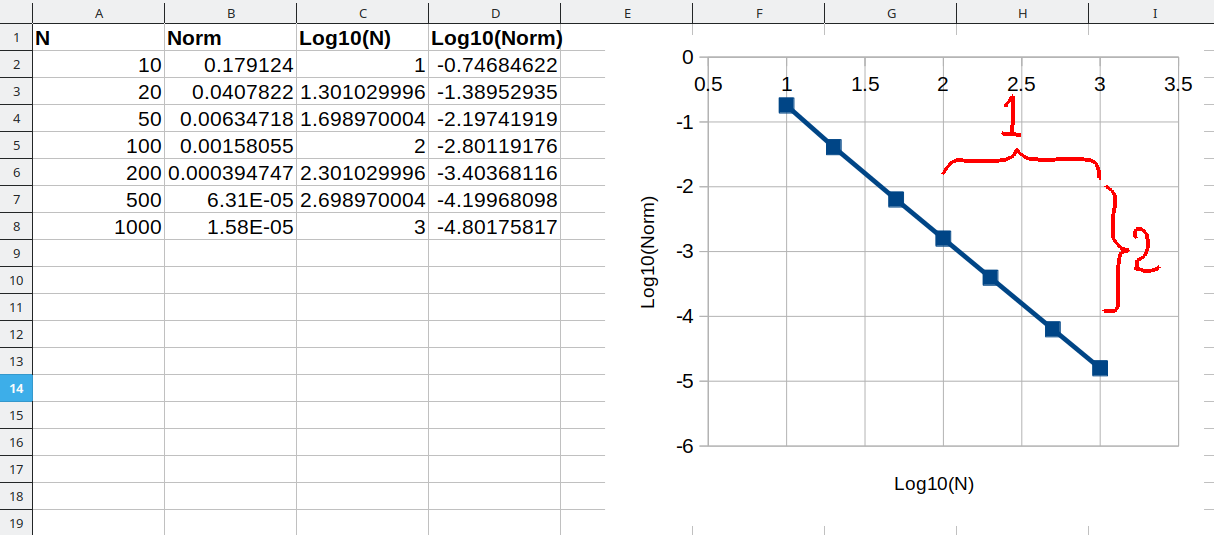
\includegraphics[width=0.9\linewidth]{poisson1_appr.png}
\caption{Сходимость с уменьшением разбиения при решении одномерного уравнения Пуассона}
\label{fig:poisson_convergence}
\end{figure}

Открыв один из cохранённых в процессе работы файлов vtk \ename{poisson1_ncells=?.vtk} в paraview
можно посмотреть полученные графики. В файле представлены как точное ``exact'', так и численное решение ``numerical''
(\figref{fig:poisson_graph}).

\begin{figure}[h]
\centering
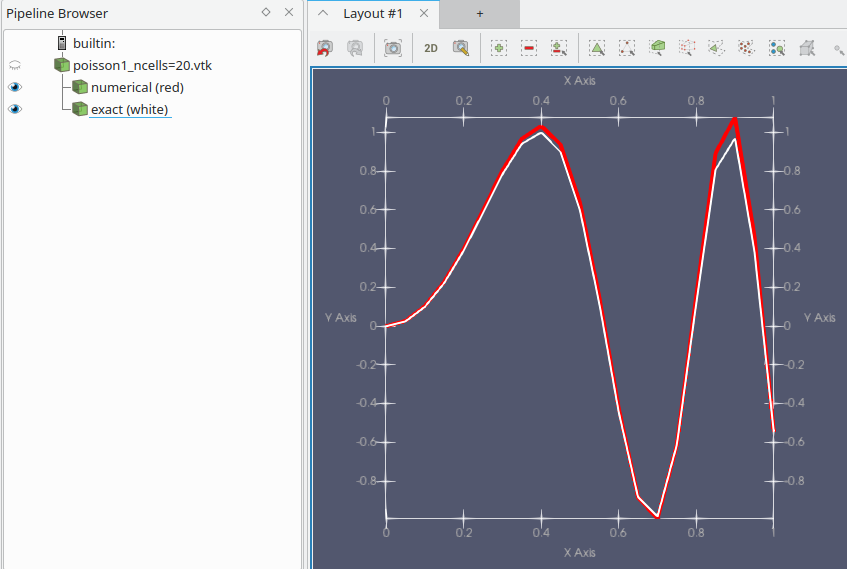
\includegraphics[width=0.9\linewidth]{poisson1_graph.png}
\caption{Сравнение точного и численного решений уравнения Пуассона}
\label{fig:poisson_graph}
\end{figure}


\subsubsubsection{Детали реализации}
\clisting{open}{"test/poisson_fdm_test.cpp"}
Основная работа по решению задачи проводится в классе \cvar{TestPoisson1Worker}.

В его конструкторе происходит инициализация сетки (приватного поля класса) на отрезке $[0, 1]$ с заданным разбиением
\cvar{n_cells}:
\clisting{line}{"TestPoisson1Worker"}

В методе \cvar{solve()} производится чиленное решения задачи и вычисления нормы.
Для этого последовательно
\begin{enumerate}
\item Строится матрица левой части и вектор правой части определяющей системы уравнений.
      Матрицы хранятся в разреженном формате CSR, удобном для последовательного чтения.
\item Вызывается решатель СЛАУ. Решение записывается в приватное поле класса \cvar{u}.
\item Вызывается функция вычисления нормы.
\end{enumerate}

\clisting{block}{"double solve()"}

Функции нижнего уровня (используемые в методе \cvar{solve}):
\begin{itemize}
\item
  Сборка левой части СЛАУ. Реализует формулу \eqref{eq:poisson1d_fdm_lhs}.
  Для заполнения матрицы используется формат \cvar{cfd::LodMatrix}, удобный для непоследовательной записи, который в конце конвертируется CSR.
  \clisting{block}{"approximate_lhs("}
\item
  Сборка правой части СЛАУ. Реализует формулу \eqref{eq:poisson1d_fdm_rhs}.
  \clisting{block}{"approximate_rhs("}
\item
  Вычисление нормы. Реализует формулу \eqref{eq:poisson1d_fdm_norm}.
  \clisting{block}{"compute_norm2"}
\end{itemize}

\subsection{Метод конечных объёмов}
\label{sec:FVM}
Будем рассматривать задачу в многомерной постановке \cref{eq:poissonnd,eq:poissonnd_bc}.

\subsubsection{Конечнообъёмная сетка}
Разобъём oбласть численного решения на на непересекающиеся подобласти $E_i$, $i = \overline{0, N-1}$,
а её границу $\partial \Omega$ на грани $\Gamma_s$, $s = \overline{0, N^\Gamma - 1}$ (\figref{fig:fvm_grid}).
Введем следующие сеточные примитивы:
\begin{itemize}
\item $E_i$ -- ячейка сетки,
\item $\Gamma_{s}$ -- граничная грань,
\item $\vec c_i$ -- центр (масс) ячейки,
\item $\vec g_s$ -- центр (масс) грани $\Gamma_{is}$.
\item $\gamma_{ij}$ -- внутренняя грань между $i$-ой и $j$-ой ячейками,
\end{itemize}
Будем считать, что ячейки сетки выпуклые, а грани -- плоские.

\begin{figure}[h!]
\centering
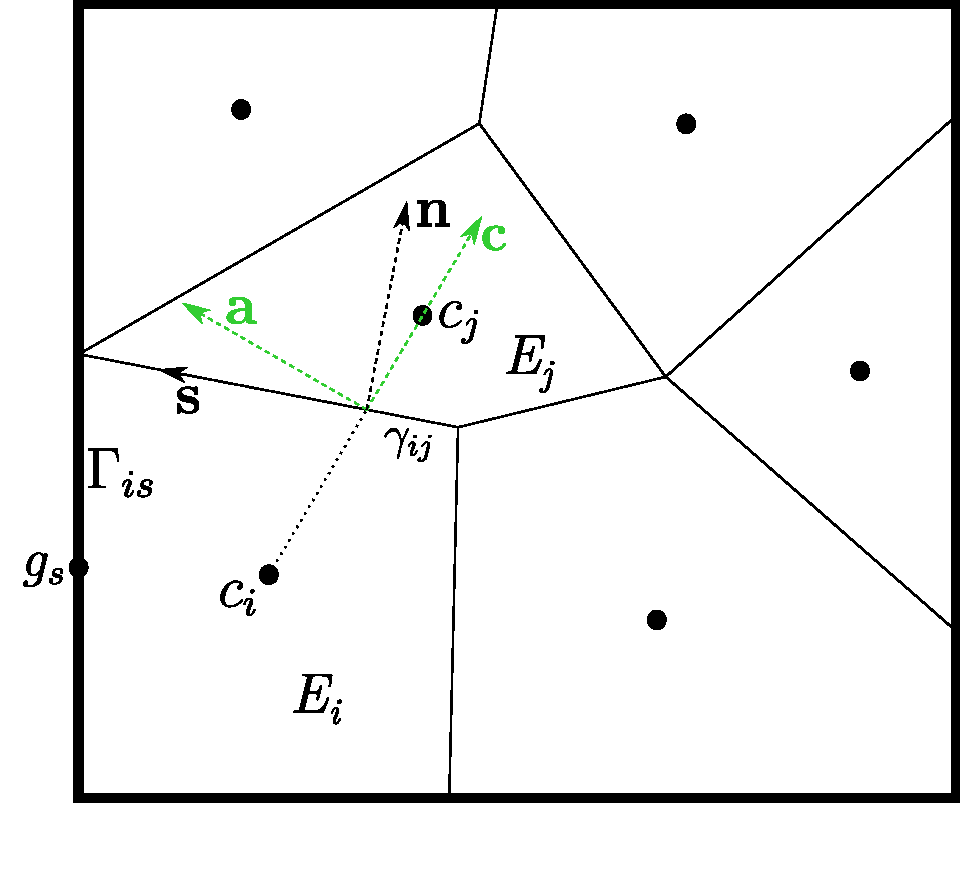
\includegraphics[width=0.4\linewidth]{fvm_grid.pdf}
\caption{Конечнообъёмная сетка}
\label{fig:fvm_grid}
\end{figure}

\subsubsection{Конечнообъёмная аппроксимация}

Проинтегрируем исходное уравнение по одной из подобластей $E_i$:
\begin{equation*}
-\arint{\nabla^2 u}{E_i}{s} = \arint{f}{E_i}{\vec x}.
\end{equation*}
К интегралу в левой части применим формулу интегрирования по частям \cref{eq:partint_laplace}. Получим
\begin{equation}
\label{eq:fvm_pois_int}
-\arint{\dfr{u}{n}}{\partial E_i}{s} = \arint{f}{E_i}{\vec x}.
\end{equation}
Здесь $\partial E_i$ -- совокупность всех границ подобласти $E_i$,
а $\vec n$ -- внешняя к подобласти нормаль.

Граница ячейки $E_i$ состоит из внутренних граней $\gamma_{ij}$ (индекс $j$ здесь
соответствует индексу соседней ячейки)
и инцидентных ей граней $\Gamma_{s}$, лежащих на внешней границе расчётной области $\Omega$.
Тогда интеграл по общей границе ячейки распишется через сумму интегралов по плоским поверхностям
$$
\arint{\dfr{u}{n}}{\partial E_i}{s} = \sum_j\arint{\dfr{u}{n}}{\gamma_{ij}}{s} + \sum_s\arint{\dfr{u}{n}}{\Gamma_{s}}{s}.
$$
Аппроксимирум производную $\dsfr{u}{n}$ на каждой из граней константой.
Тогда её можно вынести из под интегралов и предыдущее выражение записать в виде
\begin{equation}
\label{eq:fvm_gamma_integral}
\arint{\dfr{u}{n}}{\partial E_i}{s} \approx
\sum_j
    \left|
        \gamma_{ij}
    \right|
    \left(
        \dfr{u}{n}
    \right)_{\gamma_{ij}}
+\sum_s
    \left|
        \Gamma_{s}
    \right|
    \left(
        \dfr{u}{n}
    \right)_{\Gamma_{is}}
\end{equation}

Аналогично, анализируя интеграл правой части \cref{eq:fvm_pois_int},
приблизим значение функции правой части $f$ внутри элемента $E_i$ константой $f_i$,
которую отнесём к центру элемента. Тогда
\begin{equation}
\label{eq:fvm_f_integral}
\arint{f}{E_i}{\vec x} \approx f_i \left|E_i\right|.
\end{equation}

Сеточный вектор $\{f_i\}$ -- есть конечнообъёмная аппроксимация
функции $f(\vec x)$ на конечнообъёмную сетку.
Значения $f_i$ при аппроксимации чаще всего находятся как значения в центрах элементов
$$
f_i = f(\vec c_i).
$$
Хотя иногда может быть использовано и другое определение,
следующее из \eqref{eq:fvm_f_integral}:
$$
f_i = \frac{1}{\left| E_i \right|} \arint{f(\vec x)}{E_i}{\vec x}.
$$


\subsubsubsection{Обработка внутренних граней}
Для начала будем рассматривать сетки, в
которых вектора $\vec c$, соединяющие центры ячеек (зедёные вектора на \figref{fig:fvm_grid}),
коллинеарны (или почти коллинеарны) нормалям к граням $\vec n$.
В этом случае производную искомой функции по нормали к грани можно записать в виде
$$
\dfr{u}{n} = \dfr{u}{c}.
$$

Далее определим значения функции $u$ в точках $c_i$, $c_j$ как $u_i$, $u_j$.
Тогда значение производной $\dsfr{u}{n}$ на внутренней грани конечного объёма
может быть приближена конечной разностью
\begin{equation}
\label{eq:fvm_dudn_dudc}
\dfr{u}{n} = \dfr{u}{c} \approx \frac{u_j - u_i}{h_{ij}}, \quad h_{ij} = |\vec c_j - \vec c_i|.
\end{equation}

Определим pebi (perpendicular-bisector) сетки как сетки, удовлетворяющие следующим свойствам
\begin{itemize}
\item линии, соединяющие центры двух соседних ячеек, перпендикулярны грани между этими ячейками;
\item внутренние грани делят линии, соединящие центры соседних ячеек, пополам.
\end{itemize}
Очевидно, что равномерная структурированная сетка удовлетворяет этим свойствам.
Для построения неструктурированных pebi-сеток используют алгоритмы построения ячеек Вороного.
Для pebi-сеток разностная схема \eqref{eq:fvm_dudn_dudc}
является симметричной разностью и, поэтому, имеет второй порядок аппроксимации.

\subsubsubsection{Учёт граничных условий первого рода}
Для вычисления второго слагаемого в правой части 
\cref{eq:fvm_gamma_integral}
следует расписать значение нормальной 
к границе производной вида
$$
\left(\dfr{u}{n}\right)_{\Gamma_{s}}.
$$
Это делается с помощью граничных условий.

Пусть в центре $\vec g_s$ грани $\Gamma_{s}$ задано 
значение искомой функции \cref{eq:poissonnd_bc}:
\begin{equation}
\label{eq:fvm_bc1}
u(\vec g_s) = u^\Gamma_s.
\end{equation}
Аппроксимацию производных
будем проводить из тех же соображений, которые использовали
при анализе внутренних граней. Только вместо центра соседнего элемента
$c_j$ будем использовать центр грани $g_s$.
В первом приближении, отбрасывая касательные производные, придём к формуле аналогичной \cref{eq:fvm_dudn_dudc}:
\begin{equation}
\label{eq:fvm_bc1_approx}
\dfr{u}{n} \approx \frac{u^\Gamma_s - u_i}{h_{is}}, \quad h_{is} = \left| \vec g_s  - \vec c_i \right|.
\end{equation}

\subsubsection{Одномерный случай}
Рассмотрим результат конечнообъёмной аппроксимации
задачи \cref{eq:poissonnd} в одномерном случае \cref{eq:poisson1d}
на равномерной сетке с шагом $h$ (\figref{fig:fvm_grid1d}).

\begin{figure}[h!]
\centering
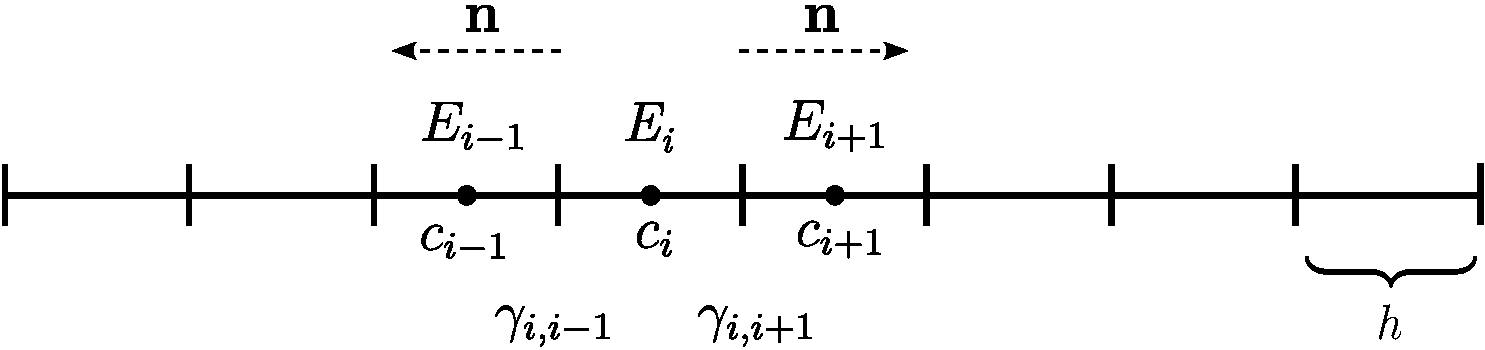
\includegraphics[width=0.6\linewidth]{fvm_grid1d.pdf}
\caption{Одномерная конечнообъёмная сетка}
\label{fig:fvm_grid1d}
\end{figure}

У внутренней ячейки $i$ есть две границы: $\gamma_{i,i-1}$ и $\gamma_{i,i+1}$.
Нормали по этим границам аппроксимируются по формулам \cref{eq:fvm_dudn_dudc}:
\begin{align*}
\gamma_{i,i-1}: \quad& \dfr{u}{n} = \frac{u_{i-1}-u_{i}}{h} \\[10pt]
\gamma_{i,i+1}: \quad& \dfr{u}{n} = \frac{u_{i+1}-u_{i}}{h}
\end{align*}
Объём ячейки в одномерном случае равен её длине $h$.
Площадь грани следует положить единице с тем, чтобы
$$
|E_i| = |\gamma| h = h.
$$
Тогда, подставляя эти значения в \cref{eq:fvm_pois_int},
получим знакомую конечноразностную схему аппроксимацию уравнения Пуассона
$$
\frac{-u_{i-1} + 2 u_i - u_{i+1}}{h} = f_i h,
$$
которая имеет второй порядок точности.
Разница с методом конечных разностей здесь состоит в том,
что значения сеточных векторов $\gvec{u}$, $\gvec{f}$ здесь
приписаны к центрам ячеек, а не к их узлам.
Это отличие проявит себя в аппроксимации граничных условий.
Так, если на левой границе $x=a$ задано условие первого рода, то соответствующее уравнение
согласно \cref{eq:fvm_bc1_approx}
примет вид
$$
-\frac{u^\Gamma_a - u_0}{h/2} - \frac{u_1 - u_0}{h} = f_0 h.
$$
В методе конечных разностей это условие выразилось бы в виде $u_0 = u^\Gamma_a$.

\subsubsection{Сборка системы линейных уравнений}
Подставим все полученные аппроксимации
\cref{eq:fvm_dudn_dudc,eq:fvm_bc1_approx}
в уравнение \cref{eq:fvm_pois_int}. Получим $i$-ое уравнение искомой системы уравнений относительно неизвестных $u_i$:
\begin{equation*}
-\sum_{j\in {\rm J}_i}
    \frac{|\gamma_{ij}|}{h_{ij}}
         \left(u_j - u_i\right)
-\sum_{s\in{\rm I}_i}
    \frac{|\Gamma_{s}|}{h_{is}}
        \left(u^\Gamma_s - u_i\right)
=
f_i |E_i|.
\end{equation*}
Введены следующие обозначения множества индексов: ${\rm J}_i$ -- индексы ячеек, соседних (имеющих общую грань) с текущей ячейкой $i$,
${\rm I}_i$ -- индексы граничных граней первого рода, инцидентных ячейке $E_i$.
Здесь первое слагаемое в левой части отвечает за потоки через внутренние границы,
второе -- граничные условия первого рода.
Далее перенесём все известные значения в правую часть и окончательно
получим линейное уравнение для $i$-го конечного объёма:
\begin{equation}
\label{eq:fvm_slae}
\sum_{j\in{\rm J}_i}
    \frac{|\gamma_{ij}|}{h_{ij}}
         \left(u_i - u_j\right)
+\sum_{s\in{\rm I}_i}
    \frac{|\Gamma_{s}|}{h_{is}}u_i
 =
f_i |E_i|
+\sum_{s\in{\rm I}_i}
    \frac{|\Gamma_{s}|}{h_{is}} u^\Gamma
\end{equation}
Таким образом мы получили систему из $N$ (по количеству подобластей) линейных уравнений относительно
неизвестного сеточного вектора $\left\{u_i\right\}$
$$
A u = b.
$$

Полученные в результате сборочных процедур матрицы являются разреженными -- то есть большинство их элементов равно нулю.
Полное хранение таких матриц в памяти невозможно, поэтому применяют специальные процедуры разреженного хранения (см. \secref{sec:sparse-matrix}).

Ниже приведён псеводкод для сборки СЛАУ. Перед началом процедур сборки левую правую часть нужно инициализировать нулями.

\subsubsubsection{Алгоритм сборки в цикле по ячейкам}
\label{sec:poisson_fvm_cellbased}
Матрицу $A$ и правую часть $b$ системы \cref{eq:fvm_slae} можно
собирать в цикле по ячейкам: строчка за строчкой.
Такой алгоритм выглядел бы следующим образом
\begin{equation*}
\begin{array}{ll}
\textbf{for } i = \overline{0, N-1}                          & \textrm{-- цикл по строкам СЛАУ}\\
\qquad b_i = |E_i| f_i                                       & \\
\qquad \textbf{for } j \in \textrm{nei(i)}                   & \textrm{-- цикл по ячейкам, соседним с ячейкой $i$}\\
\qquad \qquad v = \sfrac{|\gamma_{ij}|}{h_{ij}}              & \\
\qquad \qquad A_{ii} \pluseq v                               & \\
\qquad \qquad A_{ij} \minuseq v                              & \\
\qquad \textbf{endfor}                                       & \\
\qquad \textbf{for } s \in \textrm{bnd1(i)}                  & \textrm{-- цикл по граням ячейки $i$ с условиями первого рода}\\
\qquad \qquad v = \sfrac{|\Gamma_{is}|}{h_{is}}              & \\
\qquad \qquad A_{ii} \pluseq v                               & \\
\qquad \qquad b_{i}  \pluseq u_i^{\Gamma} v                  & \\
\qquad \textbf{endfor}                                       & \\
\textbf{endfor}
\end{array}
\end{equation*}
Первым недостатком такого алгоритма является наличие вложенных циклов.
Во-вторых, коэффициент, отвечающий за поток через внутреннюю грань $\gamma_{ij}$,
равный $\sfrac{|\gamma_{ij}|}{h_{ij}}$ в таком алгоритме будет учитываться дважды:
в строке $i$ и в строке $j$.

\subsubsubsection{Алгоритм сборки в цикле по граням}
\label{sec:poisson_fvm_facebased}
Вместо общего цикла по ячейкам, будем использовать цикл по граням.
В таком цикле коэффициенты потоков будут вычисляться один раз
и вставляться сразу в две строки матрицы, соответствующие соседним с гранью ячейкам.
Вложенных циклов в такой постановке удаётся избежать, потому
что у грани есть только две соседние ячейки (в то время как у ячейки может быть произвольное
количество соседних граней).

Разделим все грани на исходной сетки на внутренние и граничные (отдельный набор для каждого вида граничных условий).
Тогда для внутренних граней можно записать
\begin{equation}
\label{eq:fvm_assem_internal}
\begin{array}{ll}
\textbf{for } s \in\textrm{internal}                     & \textrm{-- цикл по внутренним граням}\\ 
\qquad i,j = \textrm{nei\_cells(s)}                      & \textrm{-- две ячейки, соседние с текущей гранью}\\
\qquad v = \sfrac{|\gamma_{ij}|}{h_{ij}}                 & \\
\qquad A_{ii} \pluseq  v; \quad A_{jj} \pluseq  v        & \textrm{-- диагональные коэффициенты матрицы}\\ 
\qquad A_{ij} \minuseq v; \quad A_{ji} \minuseq v        & \textrm{-- внедиагональные коэффициенты матрицы}\\
\textbf{endfor}                                          & \\
\end{array}
\end{equation}
Граничные условия учитываются в отдельных циклах.
Здесь будем учитывать, что у грани, принадлежащей
границе области, есть только одна соседняя ячейка.
Условия первого рода:
\begin{equation}
\label{eq:fvm_assem_bc1}
\begin{array}{ll}
\textbf{for } s \in\textrm{bnd1}                         & \textrm{-- грани с условиями первого рода}\\ 
\qquad i = \textrm{nei\_cells(s)}                        & \textrm{-- соседняя с граничной гранью ячейка}\\
\qquad v = \sfrac{|\Gamma_{is}|}{h_{is}}                 & \\
\qquad A_{ii} \pluseq  v                                 & \\ 
\qquad b_{i} \pluseq u_i^\Gamma v                        & \\
\textbf{endfor}                                          & \\
\end{array}
\end{equation}
Первое слагаемое в правой части
\cref{eq:fvm_slae}
учтём отдельным циклом:
\begin{equation}
\label{eq:fvm_assem_f}
\begin{array}{ll}                                         & \\
\textbf{for } i = \overline{0,N-1}                        & \textrm{-- цикл по ячейкам}\\ 
\qquad b_i \pluseq |E_i| f_i                              & \\
\textbf{endfor}                                           &
\end{array}
\end{equation}
